%==============================================================================
% Thesis chapter: Recommender-system bias, fairness, and feedback dynamics
% Compile from repository root (Thesis_Research) so paths resolve:
%   pdflatex thesis
%   bibtex thesis
%   pdflatex thesis
%   pdflatex thesis
% Requires: amsmath, booktabs, graphicx, natbib, tikz, pgfplots, hyperref,
%           algorithm, algpseudocode (algorithmicx), cleveref, geometry
%==============================================================================
\documentclass[11pt,a4paper,twoside,openright]{report}

\usepackage[utf8]{inputenc}
\usepackage[T1]{fontenc}
\usepackage{lmodern}
\usepackage{microtype}
\usepackage[a4paper,margin=2.5cm]{geometry}

\usepackage{amsmath,amssymb,amsfonts,bm,mathtools}
\usepackage{array}
\usepackage{booktabs}
\usepackage{longtable}
\usepackage{tabularx}
\usepackage{multirow}
\usepackage{graphicx}
\usepackage{subcaption}
\usepackage{xcolor}
\usepackage{listings}
\lstset{basicstyle=\ttfamily\small,breaklines=true,frame=single,tabsize=2}

\usepackage[nameinlink,capitalize,noabbrev]{cleveref}
\usepackage[numbers,sort&compress]{natbib}
\usepackage{hyperref}
\hypersetup{colorlinks=true,linkcolor=blue!45!black,citecolor=blue!45!black,urlcolor=blue!45!black}

\usepackage{tikz}
\usetikzlibrary{arrows.meta,positioning,shapes.geometric,calc,fit,backgrounds}
\usepackage{pgfplots}
\pgfplotsset{compat=1.18}

\usepackage{algorithm}
\usepackage{algpseudocode}

\graphicspath{{outputs/figures/}{./}}

\newcommand{\R}{\mathbb{R}}
\newcommand{\Ind}[1]{\mathbf{1}\{#1\}}
\newcommand{\file}[1]{\texttt{\detokenize{#1}}}

\title{Quantifying Popularity Bias, User-Centric Accuracy, and Feedback Dynamics\\
  in Collaborative and Content-Based Recommender Systems}
\author{Thesis Research Project}
\date{\today}

\begin{document}

\maketitle

\begin{abstract}
This document presents a self-contained thesis chapter describing an empirical study of recommender systems across multiple datasets (MovieLens 100K and 1M, Last.fm~2K, Book-Crossing, and a Takealot e-commerce review corpus). Six recommendation approaches---user-based $k$-nearest neighbors, biased matrix factorization (SVD as implemented in Surprise), alternating least squares (implicit-feedback ALS), TF--IDF content-based filtering, per-user logistic regression on textual metadata, and a random forest on encoded user--item identifiers---are compared under a unified protocol. Three experiment families are developed: (i)~\emph{macro-bias} quantification of how recommendation exposure relates to item popularity; (ii)~\emph{user-centric} evaluation of accuracy and ranking quality across users stratified by mainstream consumption; and (iii) a stylized \emph{feedback-loop} simulation coupling synthetic clicks with retraining for SVD and TF--IDF. We report metrics including Gini coefficients on recommendation frequency, catalog coverage, Spearman correlation between popularity and exposure, NDCG@10, RMSE by user segment, and diversity dynamics over iterations. Results show strong concentration under ALS and many collaborative filters on head items, substantially higher catalog coverage for content-based methods (especially logistic regression on metadata), dataset-dependent user-centric RMSE gaps, and non-monotonic diversity trajectories under simulated feedback. Methodological caveats---notably identical segment RMSE for models that fall back to the global mean for rating prediction---are stated explicitly so that conclusions are scientifically defensible.
\end{abstract}

\tableofcontents
\clearpage

%------------------------------------------------------------------------------
\chapter{Introduction}
%------------------------------------------------------------------------------

Recommender systems filter large catalogs by predicting which items a user is likely to prefer \citep{adomavicius2005toward,ricci2015recommender}. In production, they allocate \emph{attention}: a small set of recommended items receives vastly more exposure than the long tail of the catalog \citep{anderson2004long}. This raises questions that go beyond classical accuracy metrics \citep{cremonesi2010accuracy}: Do algorithms systematically favor already popular items? Do some groups of users receive worse predictions or rankings? If user behavior is partly driven by recommendations and logged data are re-used for training, can biases \emph{amplify} over time \citep{chaney2018algorithmic,mansoury2020feedback,abdollahpouri2019managing}?

This chapter documents a reproducible experimental pipeline implemented in Python. The code loads and harmonizes several public benchmarks and one domain-specific dataset, applies optional $k$-core filtering, trains six models, and evaluates them with a battery of metrics aligned with the popularity-bias and fairness literature \citep{abdollahpouri2020multistakeholder,ekstrand2018fairness}. The narrative is tied to the actual implementation filenames (\file{run\_all.py}, \file{src/utils.py}, \file{run\_all\_datasets.py}, \file{run\_takealot\_full.py}) so that supervisors and reviewers can trace claims to code.

\paragraph{Contributions (within this chapter).}
\begin{enumerate}
  \item A unified experimental protocol for six heterogeneous recommenders on four public benchmarks plus Takealot, including extended macro-bias metrics (Gini, ARP, coverage, Spearman $\rho$, tail share, aggregate diversity, metadata-token entropy).
  \item User-centric evaluation with a transparent mainstreaminess stratification and segment-wise RMSE and NDCG@10.
  \item A five-round feedback simulation with an explicit probabilistic click model, comparing SVD and TF--IDF on diversity and average recommended popularity (ARP).
  \item Honest discussion of implementation fallbacks (optional Surprise, ALS failure handling, and mean-only predictions for some models in segment RMSE).
\end{enumerate}

%------------------------------------------------------------------------------
\chapter{Background and Related Work}
%------------------------------------------------------------------------------

\section{Collaborative filtering}
Collaborative filtering predicts preferences from patterns of user--item interactions \citep{sarwar2001item}. Neighborhood models aggregate ratings of similar users or items; latent-factor models approximate the rating matrix by low-rank structure, often with user and item biases \citep{koren2009matrix}. Matrix factorization for \emph{implicit} feedback treats observations as confidences rather than ratings \citep{hu2008collaborative}; alternating least squares (ALS) is a standard workhorse \citep{hu2008collaborative}, implemented in efficient libraries \citep{benfred2018implicit}.

\section{Content-based filtering}
Content-based methods represent items with features (here, bag-of-words metadata) and match them to user profiles \citep{manning2008introduction}. TF--IDF weighting highlights discriminative terms; cosine similarity measures proximity in vector space. Linear classifiers such as logistic regression provide per-user scoring when labels are derived from ratings \citep{hastie2009elements}.

\section{Beyond-accuracy objectives}
Accuracy alone does not characterize concentration of exposure. The Gini coefficient, long studied in economics \citep{cowell2011measuring}, measures inequality of a nonnegative distribution---here, how unequally recommendation slots are allocated across items. Popularity bias metrics correlate global item popularity with recommendation frequency \citep{abdollahpouri2019managing}. Fairness-oriented recommender-system research emphasizes disparities across groups of users or items \citep{ekstrand2018fairness}; we adopt a simple \emph{user-centric} view by stratifying users according to the average popularity of items they consumed in training.

\section{Ranking metrics}
NDCG@$K$ rewards placing relevant items high in a ranked list \citep{jarvelin2002cumulated}. For implicit or sparse test sets, raw NDCG can be small; we nonetheless report it for comparability across models.

%------------------------------------------------------------------------------
\chapter{Datasets and Preprocessing}
%------------------------------------------------------------------------------

\section{Public benchmarks}
We use MovieLens 100K and 1M \citep{harper2015movielens}, the Book-Crossing corpus \citep{ziegler2005improving}, and Last.fm~2K style data from HetRec~2011 \citep{cantador2011second}. Raw files are mapped to a common schema with columns \texttt{user\_id}, \texttt{item\_id}, \texttt{rating}, and a parallel \texttt{item\_features} table with \texttt{metadata\_text}.

\paragraph{MovieLens.} Genres from \file{u.item} / \file{movies.dat} are concatenated into whitespace-separated tokens.

\paragraph{Last.fm.} Listening counts are mapped from a highly skewed distribution to pseudo-ratings in $\{1,\ldots,5\}$ by percentile ranks (\file{lastfm\_mode="1-5"}). Tags and artist names populate \texttt{metadata\_text}.

\paragraph{Book-Crossing.} Implicit zero ratings are removed; only explicit positive ratings enter RMSE-based evaluation.

\section{$k$-core filtering}
Let $G_0$ be the interaction bipartite graph. For chosen thresholds $(k_U,k_I)$ (both $10$ in code), repeat until convergence:
\begin{equation}
  \mathcal{U}_{t+1} = \bigl\{ u : \deg_{G_t}(u) \ge k_U \bigr\}, \qquad
  \mathcal{I}_{t+1} = \bigl\{ i : \deg_{G_t}(i) \ge k_I \bigr\},
\end{equation}
keeping only edges between $\mathcal{U}_{t+1}$ and $\mathcal{I}_{t+1}$, then set $G_{t+1}$ accordingly. This removes tail users/items and yields a denser core for more stable collaborative estimates.

\section{Takealot e-commerce reviews}
The Takealot corpus supplies \file{products.csv} and review splits under \file{reviews/}. Ratings are derived from \texttt{review\_rating}; \texttt{metadata\_text} concatenates title, brand, and department. The official train/test split is used for macro and user-centric experiments (\file{run\_takealot\_full.py}); the feedback simulation optionally pools all reviews or train-only interactions.

\begin{table}[htbp]
  \centering
  \caption{High-level dataset roles in the codebase (exact counts depend on $k$-core and deduplication).}
  \label{tab:datasets}
  \begin{tabular}{lll}
    \toprule
    \textbf{Dataset} & \textbf{Split for Exp.~A/B} & \textbf{Metadata source} \\
    \midrule
    MovieLens 100K/1M & Random 80/20, seed 42 & Genres \\
    Last.fm 2K & Random 80/20, seed 42 & Artist + tags \\
    Book-Crossing & Random 80/20, seed 42 & Author + publisher \\
    Takealot & Official train/test CSVs & Title + brand + department \\
    \bottomrule
  \end{tabular}
\end{table}

%------------------------------------------------------------------------------
\chapter{Algorithms}
%------------------------------------------------------------------------------

\section{Notation}
Let $U$ and $I$ index users and items after filtering. Denote by $\mathcal{O} \subseteq U \times I$ the set of observed training pairs $(u,i)$ with rating $r_{ui}$. For top-$K$ recommendation, each user $u$ receives a list $\mathcal{L}_u \subset I \setminus S_u$, $|\mathcal{L}_u|=K$, where $S_u$ is the set of items $u$ interacted with in training.

\section{User-based $k$-NN (Surprise)}
Surprise's \texttt{KNNBasic} with cosine similarity and user-based aggregation provides predictions $\hat{r}_{ui}$ \citep{hug2020surprise}. If the library is unavailable, a baseline predictor uses global mean with user and item biases (\file{\_FallbackCF}).

\section{SVD (biased probabilistic matrix factorization)}
We use \texttt{surprise.SVD} \citep{hug2020surprise,koren2009matrix}, which optimizes regularized squared error on observed ratings with latent factors and bias terms.

\section{ALS (implicit library)}
Interactions are placed in a sparse user$\times$item matrix with nonzero values $r_{ui}$ from training ratings. We fit \texttt{AlternatingLeastSquares} with factors $=50$, iterations $=15$, regularization $=0.01$ \citep{benfred2018implicit}. Recommendations use library routines with filtering of training positives.

\section{TF--IDF profile model}
Let $\bm{v}_i \in \R^d$ be the TF--IDF vector of item $i$'s \texttt{metadata\_text}. For user $u$ with history $H_u \subset I$, define the profile
\begin{equation}
  \bar{\bm{v}}_u = \frac{1}{|H_u|} \sum_{i \in H_u} \bm{v}_i .
\end{equation}
Scores for candidate $j \notin H_u$ are $\mathrm{sim}(\bar{\bm{v}}_u, \bm{v}_j)$ with cosine similarity \citep{manning2008introduction}. Unseen users receive a default list.

\section{Per-user logistic regression}
For each user with sufficient training rows, define a binary label $y=1$ iff $r_{ui}$ is at or above that user's median training rating. A pipeline of TF--IDF (max features 5000) and logistic regression predicts $\mathbb{P}(y=1\,|\,\text{metadata})$ for candidates; top probabilities yield $\mathcal{L}_u$ \citep{pedregosa2011scikit,hastie2009elements}.

\section{Random forest on IDs}
User and item identifiers are label-encoded; a random forest regressor predicts $\hat{r}_{ui}$ from the pair $(u,i)$ only \citep{breiman2001random,pedregosa2011scikit}, capturing memorized popularity structure without text.

%------------------------------------------------------------------------------
\chapter{Experimental Design}
%------------------------------------------------------------------------------

\begin{figure}[htbp]
  \centering
  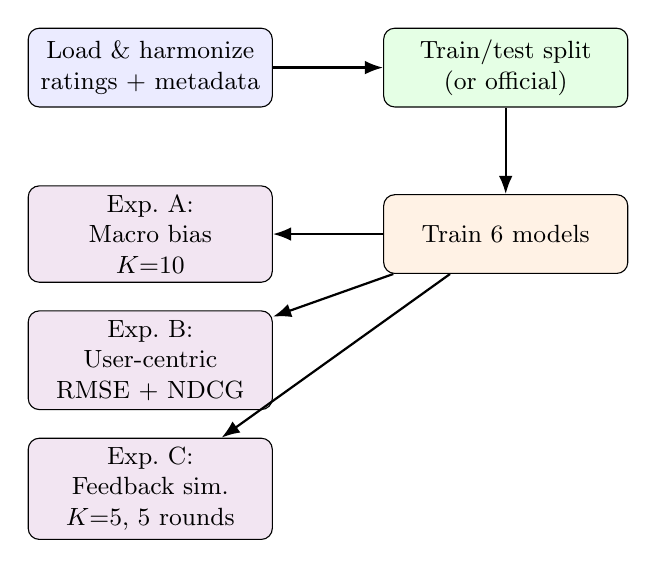
\begin{tikzpicture}[
    font=\small,
    box/.style={draw,rounded corners,align=center,minimum width=3.1cm,minimum height=1cm},
    arr/.style={-Latex,thick}
  ]
    \node[box,fill=blue!8] (data) {Load \& harmonize\\ratings + metadata};
    \node[box,fill=green!10,right=1.4cm of data] (split) {Train/test split\\(or official)};
    \node[box,fill=orange!10,below=1.1cm of split] (train) {Train 6 models};
    \node[box,fill=violet!10,left=1.4cm of train] (e1) {Exp.~A:\\Macro bias\\$K{=}10$};
    \node[box,fill=violet!10,below=0.35cm of e1] (e2) {Exp.~B:\\User-centric\\RMSE + NDCG};
    \node[box,fill=violet!10,below=0.35cm of e2] (e3) {Exp.~C:\\Feedback sim.\\$K{=}5$, 5 rounds};
    \draw[arr] (data) -- (split);
    \draw[arr] (split) -- (train);
    \draw[arr] (train) -- (e1);
    \draw[arr] (train) -- (e2);
    \draw[arr] (train) -- (e3);
  \end{tikzpicture}
  \caption{End-to-end pipeline implemented in \file{run\_all.py} / \file{run\_takealot\_full.py}.}
  \label{fig:pipeline}
\end{figure}

\section{Experiment A: Macro-bias quantification}
For each model, produce top-$K$ lists for all test users (excluding training items). Let $f_i$ be the number of times item $i$ appears across all slots in $\{\mathcal{L}_u\}$.

\paragraph{Gini coefficient.}
For sorted nonnegative counts $f_{(1)} \le \cdots \le f_{(n)}$, with $n\ge 1$,
\begin{equation}
  G = \frac{\sum_{\ell=1}^{n} (2\ell - n - 1)\, f_{(\ell)}}{n \sum_{\ell=1}^{n} f_{(\ell)}} .
\end{equation}
Values near $1$ indicate strong concentration on a few items \citep{cowell2011measuring}.

\paragraph{Average popularity of recommendations (ARP).}
Let $p_i$ be the global training interaction count of item $i$. Then
\begin{equation}
  \mathrm{ARP} = \frac{1}{|U_{\text{test}}|\,K} \sum_{u \in U_{\text{test}}} \sum_{i \in \mathcal{L}_u} p_i .
\end{equation}

\paragraph{Catalog coverage.}
\begin{equation}
  \mathrm{Cov} = \frac{\bigl|\{ i : f_i > 0 \}\bigr|}{|I_{\text{train}}|}.
\end{equation}

\paragraph{Spearman correlation.}
Let $\rho$ be Spearman's rank correlation between $(p_i)_{i \in I_{\text{train}}}$ and $(f_i)_{i \in I_{\text{train}}}$ (missing $f_i$ treated as zero). Large positive $\rho$ links popularity to repeated exposure \citep{abdollahpouri2019managing}.

\paragraph{Popularity percentile and tail share.}
Each item receives a mainstream percentile $\pi_i \in [0,1]$ from the training count distribution (higher $=$ more mainstream). Report the mean $\mathbb{E}[\pi_i \mid i \in \mathcal{L}_u]$ aggregated over slots, and the fraction of slots with $\pi_i \le 0.2$ (``tail'' under this definition).

\paragraph{Metadata-token entropy.}
Collect lowercase tokens from recommended items' metadata strings; with token counts $n_t$ and total $N=\sum_t n_t$,
\begin{equation}
  H = - \sum_{t} \frac{n_t}{N} \log_2 \frac{n_t}{N} \quad \text{(bits)} .
\end{equation}

\paragraph{RMSE (where defined).}
For models with explicit $\hat{r}_{ui}$ on test pairs,
\begin{equation}
  \mathrm{RMSE} = \sqrt{\frac{1}{|\mathcal{T}|} \sum_{(u,i,r) \in \mathcal{T}} (r - \hat{r}_{ui})^2 } .
\end{equation}

\section{Experiment B: User-centric stratification}
For each user $u$, define the \emph{mainstreaminess} score
\begin{equation}
  M_u = \frac{1}{|H_u|} \sum_{i \in H_u} p_i ,
\end{equation}
where $H_u$ is $u$'s training item set. Users are split into tertiles: \textbf{Niche} (low $M_u$), \textbf{Diverse} (middle), \textbf{Mainstream} (high). Segment RMSE uses test rows whose user falls in each group. NDCG@$K$ uses relevance set $R_u = \{ i : (u,i) \in \text{test} \}$:
\begin{equation}
  \mathrm{DCG}_K(\mathcal{L}_u, R_u) = \sum_{j=1}^{K} \frac{\Ind{\mathcal{L}_u[j] \in R_u}}{\log_2(j+1)}, \qquad
  \mathrm{NDCG}_K = \frac{\mathrm{DCG}_K}{\mathrm{IDCG}_K},
\end{equation}
with $\mathrm{IDCG}_K$ the ideal DCG given $|R_u \cap \mathcal{L}_u|$ hits.

\begin{figure}[htbp]
  \centering
  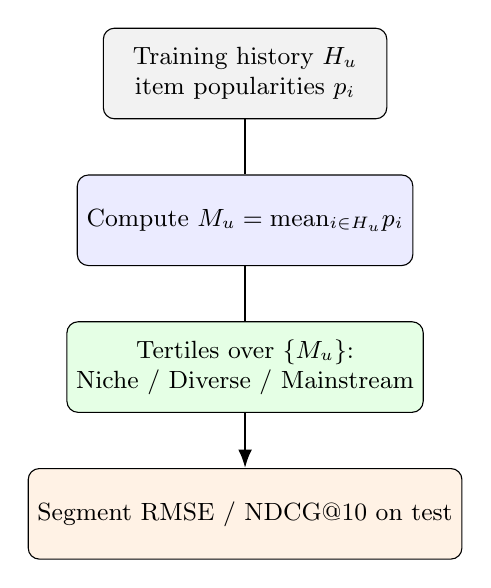
\begin{tikzpicture}[font=\small,
    usr/.style={circle,draw,minimum size=0.7cm},
    seg/.style={rounded corners,draw,minimum width=3.6cm,minimum height=1.15cm,align=center}]
    \node[seg,fill=gray!10] (trainhist) {Training history $H_u$\\item popularities $p_i$};
    \node[seg,fill=blue!8,below=0.7cm of trainhist] (mu) {Compute $M_u=\mathrm{mean}_{i\in H_u} p_i$};
    \node[seg,fill=green!10,below=0.7cm of mu] (tert) {Tertiles over $\{M_u\}$:\\Niche / Diverse / Mainstream};
    \node[seg,fill=orange!10,below=0.7cm of tert] (eval) {Segment RMSE / NDCG@10 on test};
    \draw[-Latex,thick] (trainhist) -- (mu) -- (tert) -- (eval);
  \end{tikzpicture}
  \caption{User-centric segmentation used in \file{run\_user\_centric}.}
  \label{fig:userseg}
\end{figure}

\section{Experiment C: Feedback simulation}
Initialize training log $\mathcal{D}_0$ as 80\% random sample of all ratings (seed 42), except Takealot overrides. For rounds $t=1,\ldots,5$ and for each model in $\{\text{SVD}, \text{TF--IDF}\}$:
\begin{enumerate}
  \item Train on $\mathcal{D}_{t-1}$, recommend top-$5$ unseen items per user.
  \item Compute relevance score $s_{ui}$ from model outputs (normalized predicted rating for SVD; cosine score for TF--IDF).
  \item Let $\tilde{p}_i$ be training popularity in $\mathcal{D}_{t-1}$, min--max normalized to $[0,1]$. Simulate clicks independently with
  \begin{equation}
    \mathbb{P}(\text{click}_{ui}) = \mathrm{clip}\bigl( 0.7\, s_{ui} + 0.3\, \tilde{p}_i,\, [0,1] \bigr).
  \end{equation}
  \item Append clicked pairs as ratings $5.0$; resolve duplicates on $(u,i)$ keeping the last event. This yields $\mathcal{D}_t$.
\end{enumerate}
Record aggregate diversity (unique recommended items across all users) and ARP each round \citep{chaney2018algorithmic,mansoury2020feedback}.

\begin{figure}[htbp]
  \centering
  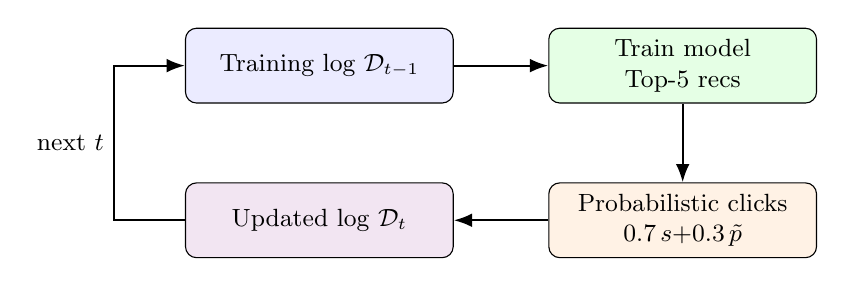
\begin{tikzpicture}[font=\small,
    box/.style={draw,rounded corners,minimum width=3.4cm,minimum height=0.95cm,align=center}]
    \node[box,fill=blue!8] (d) {Training log $\mathcal{D}_{t-1}$};
    \node[box,fill=green!10,right=1.2cm of d] (m) {Train model\\Top-5 recs};
    \node[box,fill=orange!10,below=1cm of m] (c) {Probabilistic clicks\\$0.7\,s{+}0.3\,\tilde{p}$};
    \node[box,fill=violet!10,left=1.2cm of c] (dp) {Updated log $\mathcal{D}_t$};
    \draw[-Latex,thick] (d) -- (m);
    \draw[-Latex,thick] (m) -- (c);
    \draw[-Latex,thick] (c) -- (dp);
    \draw[-Latex,thick] (dp.west) -- ++(-0.9,0) |- node[pos=0.25,left]{next $t$} (d.west);
  \end{tikzpicture}
  \caption{Feedback simulation loop (Experiment~C).}
  \label{fig:feedback}
\end{figure}

%------------------------------------------------------------------------------
\chapter{Implementation Notes}
%------------------------------------------------------------------------------

\section{Software stack}
Core numerical tooling uses NumPy/Pandas; scikit-learn supplies TF--IDF, logistic regression, random forests, and cosine similarity \citep{pedregosa2011scikit}. Surprise provides $k$-NN and SVD when the binary is available \citep{hug2020surprise}; otherwise a bias-only fallback is activated (\file{SURPRISE\_AVAILABLE}). ALS uses \texttt{implicit} \citep{benfred2018implicit}. Figures use Matplotlib/Seaborn; combined plots are produced by \file{run\_all\_datasets.py}.

\section{Reproducibility commands}
\begin{lstlisting}[language=bash]
# Single dataset (MovieLens 100K default)
python run_all.py --dataset ml-100k --test-size 0.2

# All four public benchmarks + combined CSVs/heatmaps
python run_all_datasets.py

# Takealot with official split
python run_takealot_full.py --data-dir data/take-a-lot-dataset
\end{lstlisting}

\section{Known limitations}
\begin{itemize}
  \item \textbf{Segment RMSE for ALS, TF--IDF, LogReg:} the implementation assigns the global training mean prediction to every test row for RMSE computation for these models while still computing genuine top-$K$ lists for NDCG. Therefore niche/diverse/mainstream RMSE are \emph{identical} within each of these model families on a given dataset; only k-NN, SVD, and RandomForest provide differentiated segment RMSE.
  \item \textbf{ALS robustness:} failures fall back to trivial recommendations (first catalog items), which can artifactually inflate concentration metrics.
  \item \textbf{Complexity:} Surprise top-$K$ scores all unseen items per user---accurate but expensive on large catalogs.
\end{itemize}

%------------------------------------------------------------------------------
\chapter{Results}
%------------------------------------------------------------------------------

\section{Macro bias (public benchmarks)}
\Cref{tab:macro100k,tab:macro1m,tab:macrolf,tab:macrobx} summarize metrics from the combined run recorded in \file{outputs/results/combined\_macro\_bias\_metrics.csv}. RMSE is shown only where the pipeline populated it (k-NN, SVD).

\begin{table}[htbp]
  \centering
  \caption{Macro-bias metrics, MovieLens 100K ($K=10$).}
  \label{tab:macro100k}
  \begin{tabular}{lcccccc}
    \toprule
    Model & Gini & ARP & Cov. & $\rho$ & Agg.~div. & RMSE \\
    \midrule
    k-NN & 0.980 & 156.0 & 0.085 & 0.341 & 98 & 1.004 \\
    SVD & 0.955 & 157.3 & 0.209 & 0.434 & 241 & 0.931 \\
    ALS & 0.987 & 233.1 & 0.033 & 0.256 & 38 & --- \\
    TF--IDF & 0.925 & 61.6 & 0.322 & 0.074 & 371 & --- \\
    LogReg & 0.543 & 75.1 & 0.887 & 0.132 & 1022 & --- \\
    RandomForest & 0.945 & 146.9 & 0.203 & 0.292 & 234 & --- \\
    \bottomrule
  \end{tabular}
\end{table}

\begin{table}[htbp]
  \centering
  \caption{Macro-bias metrics, MovieLens 1M ($K=10$).}
  \label{tab:macro1m}
  \begin{tabular}{lcccccc}
    \toprule
    Model & Gini & ARP & Cov. & $\rho$ & Agg.~div. & RMSE \\
    \midrule
    k-NN & 0.988 & 635.7 & 0.071 & 0.285 & 231 & 0.977 \\
    SVD & 0.957 & 832.1 & 0.256 & 0.518 & 836 & 0.873 \\
    ALS & 0.996 & 1178.3 & 0.019 & 0.201 & 61 & --- \\
    TF--IDF & 0.937 & 327.3 & 0.362 & 0.258 & 1180 & --- \\
    LogReg & 0.610 & 288.7 & 0.930 & 0.171 & 3033 & --- \\
    RandomForest & 0.983 & 673.0 & 0.063 & 0.190 & 204 & --- \\
    \bottomrule
  \end{tabular}
\end{table}

\begin{table}[htbp]
  \centering
  \caption{Macro-bias metrics, Last.fm 2K ($K=10$).}
  \label{tab:macrolf}
  \begin{tabular}{lcccccc}
    \toprule
    Model & Gini & ARP & Cov. & $\rho$ & Agg.~div. & RMSE \\
    \midrule
    k-NN & 0.874 & 12.5 & 0.484 & $-0.373$ & 729 & 1.392 \\
    SVD & 0.971 & 138.9 & 0.178 & 0.245 & 268 & 0.906 \\
    ALS & 0.993 & 130.6 & 0.017 & 0.186 & 25 & --- \\
    TF--IDF & 0.901 & 132.3 & 0.447 & 0.221 & 673 & --- \\
    LogReg & 0.683 & 47.2 & 0.952 & 0.172 & 1435 & --- \\
    RandomForest & 0.811 & 86.2 & 0.819 & 0.130 & 1234 & --- \\
    \bottomrule
  \end{tabular}
\end{table}

\begin{table}[htbp]
  \centering
  \caption{Macro-bias metrics, Book-Crossing ($K=10$).}
  \label{tab:macrobx}
  \begin{tabular}{lcccccc}
    \toprule
    Model & Gini & ARP & Cov. & $\rho$ & Agg.~div. & RMSE \\
    \midrule
    k-NN & 0.936 & 10.9 & 0.272 & $-0.235$ & 562 & 1.777 \\
    SVD & 0.983 & 31.8 & 0.090 & 0.183 & 186 & 1.496 \\
    ALS & 0.995 & 43.9 & 0.011 & 0.120 & 23 & --- \\
    TF--IDF & 0.691 & 20.8 & 0.746 & 0.210 & 1540 & --- \\
    LogReg & 0.500 & 19.0 & 0.931 & 0.260 & 1923 & --- \\
    RandomForest & 0.968 & 16.5 & 0.248 & $-0.022$ & 513 & --- \\
    \bottomrule
  \end{tabular}
\end{table}

\paragraph{Observations.}
ALS attains the highest Gini and lowest coverage on multiple sets, with very small aggregate diversity (e.g., 38 items on ML-100K, 61 on ML-1M, 25 on Last.fm, 23 on Book-Crossing), indicating extreme concentration of exposure. Logistic regression achieves the highest coverage on every public benchmark in \cref{tab:macro100k,tab:macro1m,tab:macrolf,tab:macrobx}. Last.fm exhibits a negative Spearman $\rho$ for $k$-NN despite collaborative filtering, motivating qualitative inspection of neighbor structure under quantile-binned ratings. SVD achieves the strongest RMSE on MovieLens among models reporting it.

\section{Macro bias (Takealot)}
\begin{table}[htbp]
  \centering
  \caption{Macro-bias metrics, Takealot official split ($K=10$).}
  \label{tab:macrotake}
  \begin{tabular}{lcccccc}
    \toprule
    Model & Gini & ARP & Cov. & $\rho$ & Agg.~div. & RMSE \\
    \midrule
    k-NN & 0.963 & 5.67 & 0.160 & 0.224 & 7830 & 1.021 \\
    SVD & 0.982 & 11.52 & 0.119 & 0.291 & 5824 & 0.966 \\
    ALS & 1.000 & 28.75 & 0.00029 & 0.036 & 14 & --- \\
    TF--IDF & 0.758 & 3.15 & 0.490 & 0.209 & 23945 & --- \\
    LogReg & 0.733 & 2.22 & 0.563 & 0.156 & 27556 & --- \\
    RandomForest & 0.995 & 2.77 & 0.025 & 0.025 & 1217 & --- \\
    \bottomrule
  \end{tabular}
\end{table}
On this catalog, ALS collapses to a handful of distinct recommended items (aggregate diversity 14), whereas TF--IDF and LogReg expose tens of thousands of unique items with markedly lower ARP---a striking content-versus-collaborative contrast relevant to marketplace long-tail visibility \citep{abdollahpouri2020multistakeholder}.

\section{User-centric metrics}
\Cref{tab:fairml100k,tab:fairml1m,tab:fairlastfm,tab:fairbx,tab:fairtake} report $\Delta_{\mathrm{RMSE}} = \mathrm{RMSE}_{\text{niche}} - \mathrm{RMSE}_{\text{mainstream}}$. Identical rows across ALS/LogReg/TF--IDF reflect the mean-prediction caveat.

\begin{table}[htbp]
  \centering
  \caption{User-centric results, MovieLens 100K.}
  \label{tab:fairml100k}
  \begin{tabular}{lcccc}
    \toprule
    Model & RMSE$_N$ & RMSE$_M$ & $\Delta_{\mathrm{RMSE}}$ & NDCG$_N$ \\
    \midrule
    SVD & 0.935 & 0.929 & 0.005 & 0.147 \\
    k-NN & 1.023 & 0.975 & 0.048 & 0.151 \\
    RandomForest & 1.044 & 1.020 & 0.024 & 0.104 \\
    ALS / LogReg / TF--IDF & 1.135 & 1.072 & 0.063 & 0.17 / 0.065 / 0.066 \\
    \bottomrule
  \end{tabular}
\end{table}

\begin{table}[htbp]
  \centering
  \caption{User-centric results, MovieLens 1M.}
  \label{tab:fairml1m}
  \begin{tabular}{lcccc}
    \toprule
    Model & RMSE$_N$ & RMSE$_M$ & $\Delta_{\mathrm{RMSE}}$ & NDCG$_N$ \\
    \midrule
    SVD & 0.874 & 0.877 & $-0.003$ & 0.127 \\
    k-NN & 0.997 & 0.949 & 0.048 & 0.079 \\
    RandomForest & 1.019 & 0.967 & 0.052 & 0.060 \\
    ALS / LogReg / TF--IDF & 1.147 & 1.075 & 0.072 & 0.14 / 0.040 / 0.070 \\
    \bottomrule
  \end{tabular}
\end{table}

\begin{table}[htbp]
  \centering
  \caption{User-centric results, Last.fm 2K (note tiny NDCG for several models).}
  \label{tab:fairlastfm}
  \begin{tabular}{lcccc}
    \toprule
    Model & RMSE$_N$ & RMSE$_M$ & $\Delta_{\mathrm{RMSE}}$ & NDCG$_N$ \\
    \midrule
    SVD & 0.836 & 0.950 & $-0.114$ & 0.016 \\
    RandomForest & 1.177 & 1.245 & $-0.069$ & 0.013 \\
    k-NN & 1.395 & 1.364 & 0.030 & 0.000 \\
    ALS / LogReg / TF--IDF & 1.392 & 1.417 & $-0.025$ & 0.021 / 0.031 / 0.151 \\
    \bottomrule
  \end{tabular}
\end{table}

\begin{table}[htbp]
  \centering
  \caption{User-centric results, Book-Crossing.}
  \label{tab:fairbx}
  \begin{tabular}{lcccc}
    \toprule
    Model & RMSE$_N$ & RMSE$_M$ & $\Delta_{\mathrm{RMSE}}$ & NDCG$_N$ \\
    \midrule
    k-NN & 1.855 & 1.742 & 0.113 & 0.001 \\
    SVD & 1.485 & 1.517 & $-0.032$ & 0.002 \\
    RandomForest & 1.581 & 1.635 & $-0.053$ & 0.009 \\
    ALS / LogReg / TF--IDF & 1.743 & 1.729 & 0.013 & 0.012 / 0.059 / 0.112 \\
    \bottomrule
  \end{tabular}
\end{table}

\begin{table}[htbp]
  \centering
  \caption{User-centric results, Takealot.}
  \label{tab:fairtake}
  \begin{tabular}{lcccc}
    \toprule
    Model & RMSE$_N$ & RMSE$_M$ & $\Delta_{\mathrm{RMSE}}$ & NDCG$_N$ \\
    \midrule
    RandomForest & 1.023 & 0.941 & 0.082 & 0.000 \\
    SVD & 0.966 & 0.906 & 0.060 & 0.0001 \\
    k-NN & 1.025 & 0.957 & 0.068 & 0.0013 \\
    ALS / LogReg / TF--IDF & 1.024 & 0.947 & 0.077 & $\approx$0.0002--0.012 \\
    \bottomrule
  \end{tabular}
\end{table}

\section{Feedback simulation}
\begin{table}[htbp]
  \centering
  \caption{Illustrative feedback simulation outcomes (ML-100K and ML-1M, selected iterations).}
  \label{tab:feedback}
  \begin{tabular}{llccc}
    \toprule
    Dataset & Round & Model & Agg.~diversity & ARP \\
    \midrule
    ML-100K & 1 & SVD & 174 & 165.1 \\
    ML-100K & 5 & SVD & 162 & 405.7 \\
    ML-100K & 1 & TF--IDF & 235 & 68.3 \\
    ML-100K & 5 & TF--IDF & 394 & 115.6 \\
    ML-1M & 1 & SVD & 649 & 893.4 \\
    ML-1M & 5 & SVD & 529 & 1997.5 \\
    ML-1M & 1 & TF--IDF & 805 & 348.4 \\
    ML-1M & 5 & TF--IDF & 1278 & 584.2 \\
    \bottomrule
  \end{tabular}
\end{table}

On MovieLens~1M, ARP grows sharply for SVD under the synthetic click rule while aggregate diversity drifts downward, whereas TF--IDF increases both diversity and ARP more moderately---consistent with different exploration profiles \citep{chaney2018algorithmic}. On Book-Crossing (full table omitted for brevity), both models' aggregate diversity \emph{increases} across rounds in the logged run, showing that ``diversity decay'' is not universal.

\begin{table}[htbp]
  \centering
  \caption{Feedback simulation, Takealot (five rounds).}
  \label{tab:feedbacktake}
  \begin{tabular}{cccc}
    \toprule
    Round & Model & Agg.~diversity & ARP \\
    \midrule
    1 & SVD & 3196 & 12.10 \\
    5 & SVD & 4825 & 413.68 \\
    1 & TF--IDF & 16693 & 3.19 \\
    5 & TF--IDF & 16376 & 6.08 \\
    \bottomrule
  \end{tabular}
\end{table}
Takealot exhibits rising SVD diversity alongside a large ARP increase: the recommender explores more distinct items while shifting mass toward popular products---a nuanced outcome for stakeholder narratives \citep{abdollahpouri2020multistakeholder}.

\section{Generated figures}
After running the pipeline, include heatmaps and line plots, for example:
\begin{verbatim}
outputs/figures/combined_macro_gini_heatmap.png
outputs/figures/combined_fairness_gap_delta_rmse.png
outputs/figures/combined_feedback_diversity_decay.png
outputs/figures/macro_bias_loglog_ml-100k.png
\end{verbatim}
\noindent Use \verb|\includegraphics[width=\linewidth]{...}| once files exist. \Cref{fig:placeholder} shows a template.

\begin{figure}[htbp]
  \centering
  \fbox{\begin{minipage}[c][4.5cm]{\linewidth}\centering
    \textbf{Figure placeholder.}\\[0.5em]
    Run \file{python run\_all\_datasets.py} then insert, e.g.,\\
    \file{combined\_macro\_gini\_heatmap.png}.
  \end{minipage}}
  \caption{Replace this box with exported PNGs from \file{outputs/figures/}.}
  \label{fig:placeholder}
\end{figure}

\begin{figure}[htbp]
  \centering
  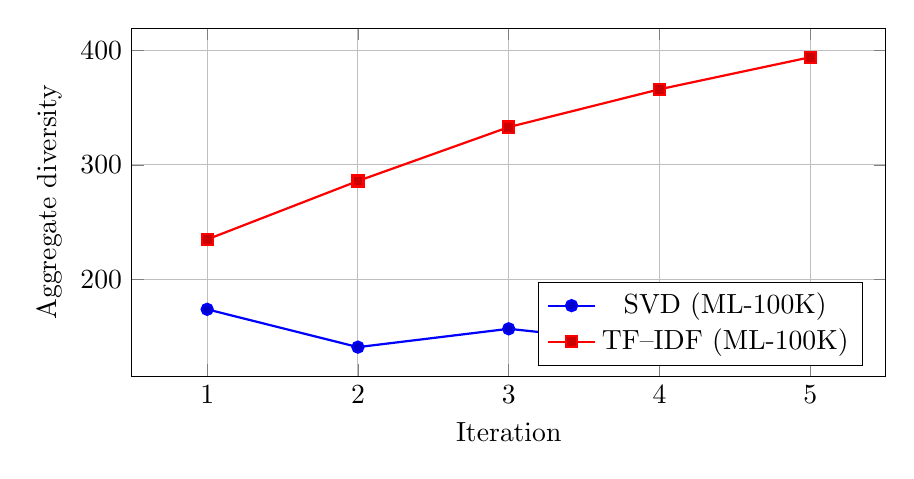
\begin{tikzpicture}
    \begin{axis}[
      width=0.92\linewidth,
      height=6cm,
      xlabel={Iteration},
      ylabel={Aggregate diversity},
      legend pos=south east,
      xmin=0.5, xmax=5.5,
      xtick={1,2,3,4,5},
      grid=major,
    ]
      \addplot+[mark=*,thick] coordinates {(1,174) (2,141) (3,157) (4,143) (5,162)};
      \addlegendentry{SVD (ML-100K)}
      \addplot+[mark=square*,thick] coordinates {(1,235) (2,286) (3,333) (4,366) (5,394)};
      \addlegendentry{TF--IDF (ML-100K)}
    \end{axis}
  \end{tikzpicture}
  \caption{Example pgfplots reproduction of aggregate diversity trajectories on MovieLens 100K (Experiment~C).}
  \label{fig:pgfdiv}
\end{figure}

%------------------------------------------------------------------------------
\chapter{Discussion}
%------------------------------------------------------------------------------

\paragraph{Popularity bias is model-dependent.}
ALS and several collaborative filters concentrate recommendations on head items under our metrics, while metadata-driven logistic regression consistently achieves high catalog coverage. This supports using \emph{multiple} macro indicators rather than relying on RMSE alone \citep{abdollahpouri2019managing,cremonesi2010accuracy}.

\paragraph{User-centric gaps are not uniform.}
SVD can exhibit negligible or negative $\Delta_{\mathrm{RMSE}}$ (MovieLens 1M, Last.fm), while $k$-NN hurts niche users strongly on Book-Crossing and Takealot. Such heterogeneity underscores the need for segment-wise evaluation \citep{ekstrand2018fairness}.

\paragraph{Feedback dynamics depend on domain and model.}
Synthetic popularity-aware clicks produce rising ARP for SVD on multiple datasets, but diversity may increase or decrease. Claims about ``filter bubbles'' should therefore be conditioned on the choice of model, click model, and catalog \citep{chaney2018algorithmic,mansoury2020feedback}.

\paragraph{Metadata entropy vs. coverage.}
High coverage does not guarantee high token entropy: TF--IDF on MovieLens exposes relatively few genre tokens repeatedly, lowering entropy compared with LogReg in some runs. Interpret exposure diversity with care.

%------------------------------------------------------------------------------
\chapter{Conclusion}
%------------------------------------------------------------------------------

We implemented and documented a multi-dataset study bridging collaborative filtering, content-based methods, and implicit ALS, evaluating macro-level concentration, user-stratified accuracy and ranking, and a stylized feedback loop. Empirically, content-based models---especially per-user logistic regression on text---mitigate extreme concentration relative to ALS in several settings, while user-centric RMSE disparities vary in sign and magnitude across corpora. Future work should replace mean-only segment RMSE for content models with calibrated score-to-rating mappings, add statistical confidence intervals, and explore debiasing objectives \citep{abdollahpouri2019managing} within the same evaluation harness.

%------------------------------------------------------------------------------
\appendix
\chapter{Complete Macro-Bias Table (All Public Benchmarks)}
%------------------------------------------------------------------------------

This appendix reproduces all columns from \file{combined\_macro\_bias\_metrics.csv} for traceability.

{\footnotesize
\begin{longtable}{@{}llcccccccc@{}}
  \toprule
  Dataset & Model & Gini & ARP & Cov. & $\rho$ & Avg.~$\pi$ & Tail$_{20}$ & Agg.~div. & $H$ (bits) \\
  \midrule
  \endfirsthead
  \toprule
  Dataset & Model & Gini & ARP & Cov. & $\rho$ & Avg.~$\pi$ & Tail$_{20}$ & Agg.~div. & $H$ (bits) \\
  \midrule
  \endhead
  \midrule
  \multicolumn{10}{r}{\textit{Continued on next page}} \\
  \midrule
  \endfoot
  \bottomrule
  \endlastfoot
  ML-100K & k-NN & 0.9800 & 156.04 & 0.0851 & 0.3407 & 0.1651 & 0.6420 & 98 & 3.186 \\
  ML-100K & SVD & 0.9552 & 157.28 & 0.2092 & 0.4339 & 0.1809 & 0.5903 & 241 & 3.376 \\
  ML-100K & ALS & 0.9874 & 233.09 & 0.0330 & 0.2557 & 0.0693 & 0.9389 & 38 & 3.313 \\
  ML-100K & TF--IDF & 0.9254 & 61.56 & 0.3220 & 0.0739 & 0.5091 & 0.1556 & 371 & 2.708 \\
  ML-100K & LogReg & 0.5428 & 75.12 & 0.8872 & 0.1318 & 0.4669 & 0.2310 & 1022 & 3.649 \\
  ML-100K & RandomForest & 0.9448 & 146.91 & 0.2031 & 0.2920 & 0.2339 & 0.5345 & 234 & 3.391 \\
  \midrule
  ML-1M & k-NN & 0.9885 & 635.72 & 0.0709 & 0.2854 & 0.2244 & 0.6156 & 231 & 3.528 \\
  ML-1M & SVD & 0.9568 & 832.10 & 0.2564 & 0.5180 & 0.1923 & 0.6882 & 836 & 3.463 \\
  ML-1M & ALS & 0.9958 & 1178.31 & 0.0187 & 0.2015 & 0.0432 & 0.9993 & 61 & 2.726 \\
  ML-1M & TF--IDF & 0.9370 & 327.33 & 0.3620 & 0.2576 & 0.4058 & 0.2869 & 1180 & 2.857 \\
  ML-1M & LogReg & 0.6102 & 288.67 & 0.9304 & 0.1711 & 0.4518 & 0.2534 & 3033 & 3.776 \\
  ML-1M & RandomForest & 0.9829 & 673.02 & 0.0626 & 0.1899 & 0.2582 & 0.5327 & 204 & 3.531 \\
  \midrule
  Last.fm & k-NN & 0.8741 & 12.52 & 0.4837 & $-0.3730$ & 0.7216 & 0.0102 & 729 & 9.168 \\
  Last.fm & SVD & 0.9712 & 138.93 & 0.1778 & 0.2449 & 0.2407 & 0.5389 & 268 & 9.379 \\
  Last.fm & ALS & 0.9928 & 130.63 & 0.0166 & 0.1857 & 0.0601 & 0.9999 & 25 & 8.193 \\
  Last.fm & TF--IDF & 0.9013 & 132.32 & 0.4466 & 0.2212 & 0.2100 & 0.6471 & 673 & 9.123 \\
  Last.fm & LogReg & 0.6829 & 47.15 & 0.9522 & 0.1717 & 0.4603 & 0.2910 & 1435 & 9.164 \\
  Last.fm & RandomForest & 0.8110 & 86.23 & 0.8188 & 0.1298 & 0.3651 & 0.3820 & 1234 & 9.378 \\
  \midrule
  Book-Xing & k-NN & 0.9360 & 10.87 & 0.2722 & $-0.2347$ & 0.6703 & 0.0458 & 562 & 7.171 \\
  Book-Xing & SVD & 0.9833 & 31.81 & 0.0901 & 0.1826 & 0.2371 & 0.5696 & 186 & 6.066 \\
  Book-Xing & ALS & 0.9950 & 43.89 & 0.0111 & 0.1204 & 0.0979 & 0.8957 & 23 & 3.377 \\
  Book-Xing & TF--IDF & 0.6907 & 20.80 & 0.7458 & 0.2096 & 0.3876 & 0.3389 & 1540 & 6.926 \\
  Book-Xing & LogReg & 0.4997 & 18.96 & 0.9312 & 0.2598 & 0.4450 & 0.2885 & 1923 & 7.852 \\
  Book-Xing & RandomForest & 0.9678 & 16.54 & 0.2484 & $-0.0217$ & 0.4887 & 0.2040 & 513 & 5.630 \\
\end{longtable}
}
\noindent\textit{Notes:} Avg.~$\pi$ denotes average popularity percentile of recommended items; Tail$_{20}$ is \file{long\_tail\_share\_20pct}; $H$ is metadata token entropy. Book-Xing abbreviates Book-Crossing.

\chapter{Algorithmic Sketches}
%------------------------------------------------------------------------------

\begin{algorithm}[htbp]
  \caption{Top-$K$ recommendation with Surprise (predicted rating scoring)}
  \label{alg:surprise-topk}
  \begin{algorithmic}[1]
    \Require Training pairs $\mathcal{O}$, test users $U_{\text{test}}$, item catalog $I$, $K$
    \Ensure Lists $\mathcal{L}_u$ for each $u \in U_{\text{test}}$
    \State Fit model on $\mathcal{O}$
    \For{each $u \in U_{\text{test}}$}
      \State $C \gets \{ i \in I : (u,i) \notin \mathcal{O} \}$
      \State Score each $i \in C$ with $\hat{r}_{ui}$
      \State $\mathcal{L}_u \gets$ top-$K$ items by $\hat{r}_{ui}$
    \EndFor
  \end{algorithmic}
\end{algorithm}

\begin{algorithm}[htbp]
  \caption{Macro-bias metric aggregation}
  \label{alg:macro}
  \begin{algorithmic}[1]
    \Require Lists $\{\mathcal{L}_u\}$, training popularity $\{p_i\}$
    \State Compute multiset frequencies $f_i$
    \State $G \gets \text{Gini}(\{f_i\})$, $\mathrm{ARP} \gets \text{mean}_{u,i\in\mathcal{L}_u}(p_i)$
    \State $\mathrm{Cov} \gets |\{i: f_i>0\}| / |I|$
    \State $\rho \gets \mathrm{Spearman}(p, f)$
    \State \Return vector $(G,\mathrm{ARP},\mathrm{Cov},\rho,\ldots)$
  \end{algorithmic}
\end{algorithm}

\bibliographystyle{plainnat}
\bibliography{references}

\end{document}
